%DIF 1-8c1-37
%DIF LATEXDIFF DIFFERENCE FILE


%DIF < \documentclass[12pt, a4paper]{article}
%DIF < \usepackage{amssymb, amsmath, amsthm}
%DIF < \usepackage{multirow}
%DIF < \usepackage{color}
%DIF < \usepackage[sort&compress]{natbib}
%DIF < \usepackage{hyperref}
%DIF < \usepackage{graphicx}
%DIF < \usepackage{setspace}
%DIF -------
% Options for packages loaded elsewhere %DIF > 
\PassOptionsToPackage{unicode}{hyperref} %DIF > 
\PassOptionsToPackage{hyphens}{url} %DIF > 
% %DIF > 
\documentclass[ %DIF > 
]{article} %DIF > 
\usepackage{amsmath,amssymb} %DIF > 
\usepackage{lmodern} %DIF > 
\usepackage{iftex} %DIF > 
\ifPDFTeX %DIF > 
  \usepackage[T1]{fontenc} %DIF > 
  \usepackage[utf8]{inputenc} %DIF > 
  \usepackage{textcomp} % provide euro and other symbols %DIF > 
\else % if luatex or xetex %DIF > 
  \usepackage{unicode-math} %DIF > 
  \defaultfontfeatures{Scale=MatchLowercase} %DIF > 
  \defaultfontfeatures[\rmfamily]{Ligatures=TeX,Scale=1} %DIF > 
\fi %DIF > 
% Use upquote if available, for straight quotes in verbatim environments %DIF > 
\IfFileExists{upquote.sty}{\usepackage{upquote}}{} %DIF > 
\IfFileExists{microtype.sty}{% use microtype if available %DIF > 
  \usepackage[]{microtype} %DIF > 
  \UseMicrotypeSet[protrusion]{basicmath} % disable protrusion for tt fonts %DIF > 
}{} %DIF > 
\makeatletter %DIF > 
\@ifundefined{KOMAClassName}{% if non-KOMA class %DIF > 
  \IfFileExists{parskip.sty}{% %DIF > 
    \usepackage{parskip} %DIF > 
  }{% else %DIF > 
    \setlength{\parindent}{0pt} %DIF > 
    \setlength{\parskip}{6pt plus 2pt minus 1pt}} %DIF > 
}{% if KOMA class %DIF > 
  \KOMAoptions{parskip=half}} %DIF > 
\makeatother %DIF > 
\usepackage{xcolor} %DIF > 
\IfFileExists{xurl.sty}{\usepackage{xurl}}{} % add URL line breaks if available %DIF > 
\IfFileExists{bookmark.sty}{\usepackage{bookmark}}{\usepackage{hyperref}} %DIF > 
%DIF -------
\hypersetup{
%DIF 10-24c39-90
%DIF <     pdftitle={Towards a standardized evaluation of multiple imputation routines}
%DIF <     pdfauthor={Gerko Vink and Andrew Gelman},
%DIF <     pdfsubject={Evaluating imputation routines},
%DIF <     pdfkeywords={Multiple imputation, evaluation, simulation, finite population},
%DIF <     bookmarksnumbered=true,     
%DIF <     bookmarksopen=true,         
%DIF <     bookmarksopenlevel=1,       
%DIF <     colorlinks=false,
%DIF <     citecolor=blue,
%DIF <     linkcolor=blue,
%DIF <     urlcolor=blue,                 
%DIF <     pdfstartview=Fit,           
%DIF <     pdfpagemode=UseOutlines,      
%DIF <     pdfpagelayout=TwoPageRight
%DIF < }
%DIF -------
  pdftitle={Towards a standardized evaluation of multiple imputation routines}, %DIF > 
  pdfauthor={Hanne Oberman and Gerko Vink}, %DIF > 
  hidelinks, %DIF > 
  pdfcreator={LaTeX via pandoc}} %DIF > 
\urlstyle{same} % disable monospaced font for URLs %DIF > 
\usepackage[margin=1in]{geometry} %DIF > 
\usepackage{graphicx} %DIF > 
\makeatletter %DIF > 
\def\maxwidth{\ifdim\Gin@nat@width>\linewidth\linewidth\else\Gin@nat@width\fi} %DIF > 
\def\maxheight{\ifdim\Gin@nat@height>\textheight\textheight\else\Gin@nat@height\fi} %DIF > 
\makeatother %DIF > 
% Scale images if necessary, so that they will not overflow the page %DIF > 
% margins by default, and it is still possible to overwrite the defaults %DIF > 
% using explicit options in \includegraphics[width, height, ...]{} %DIF > 
\setkeys{Gin}{width=\maxwidth,height=\maxheight,keepaspectratio} %DIF > 
% Set default figure placement to htbp %DIF > 
\makeatletter %DIF > 
\def\fps@figure{htbp} %DIF > 
\makeatother %DIF > 
\usepackage[normalem]{ulem} %DIF > 
% Avoid problems with \sout in headers with hyperref %DIF > 
\pdfstringdefDisableCommands{\renewcommand{\sout}{}} %DIF > 
\setlength{\emergencystretch}{3em} % prevent overfull lines %DIF > 
\providecommand{\tightlist}{% %DIF > 
  \setlength{\itemsep}{0pt}\setlength{\parskip}{0pt}} %DIF > 
\setcounter{secnumdepth}{-\maxdimen} % remove section numbering %DIF > 
\newlength{\cslhangindent} %DIF > 
\setlength{\cslhangindent}{1.5em} %DIF > 
\newlength{\csllabelwidth} %DIF > 
\setlength{\csllabelwidth}{3em} %DIF > 
\newlength{\cslentryspacingunit} % times entry-spacing %DIF > 
\setlength{\cslentryspacingunit}{\parskip} %DIF > 
\newenvironment{CSLReferences}[2] % #1 hanging-ident, #2 entry spacing %DIF > 
 {% don't indent paragraphs %DIF > 
  \setlength{\parindent}{0pt} %DIF > 
  % turn on hanging indent if param 1 is 1 %DIF > 
  \ifodd #1 %DIF > 
  \let\oldpar\par %DIF > 
  \def\par{\hangindent=\cslhangindent\oldpar} %DIF > 
  \fi %DIF > 
  % set entry spacing %DIF > 
  \setlength{\parskip}{#2\cslentryspacingunit} %DIF > 
 }% %DIF > 
 {} %DIF > 
\usepackage{calc} %DIF > 
\newcommand{\CSLBlock}[1]{#1\hfill\break} %DIF > 
\newcommand{\CSLLeftMargin}[1]{\parbox[t]{\csllabelwidth}{#1}} %DIF > 
\newcommand{\CSLRightInline}[1]{\parbox[t]{\linewidth - \csllabelwidth}{#1}\break} %DIF > 
\newcommand{\CSLIndent}[1]{\hspace{\cslhangindent}#1} %DIF > 
\ifLuaTeX %DIF > 
  \usepackage{selnolig}  % disable illegal ligatures %DIF > 
\fi %DIF > 
%DIF -------

%DIF < \singlespacing
%DIF -------
\title{\DIFaddbegin \DIFadd{Towards a standardized evaluation of multiple imputation %DIF > 
routines}\DIFaddend } %DIF > 
\author{\DIFaddbegin \DIFadd{Hanne Oberman and Gerko Vink}\DIFaddend } %DIF > 
\date{\DIFaddbegin \DIFadd{19-1-2022}\DIFaddend } %DIF > 
%DIF PREAMBLE EXTENSION ADDED BY LATEXDIFF
%DIF UNDERLINE PREAMBLE %DIF PREAMBLE
\RequirePackage[normalem]{ulem} %DIF PREAMBLE
\RequirePackage{color}\definecolor{RED}{rgb}{1,0,0}\definecolor{BLUE}{rgb}{0,0,1} %DIF PREAMBLE
\providecommand{\DIFaddtex}[1]{{\protect\color{blue}\uwave{#1}}} %DIF PREAMBLE
\providecommand{\DIFdeltex}[1]{{\protect\color{red}\sout{#1}}}                      %DIF PREAMBLE
%DIF SAFE PREAMBLE %DIF PREAMBLE
\providecommand{\DIFaddbegin}{} %DIF PREAMBLE
\providecommand{\DIFaddend}{} %DIF PREAMBLE
\providecommand{\DIFdelbegin}{} %DIF PREAMBLE
\providecommand{\DIFdelend}{} %DIF PREAMBLE
%DIF FLOATSAFE PREAMBLE %DIF PREAMBLE
\providecommand{\DIFaddFL}[1]{\DIFadd{#1}} %DIF PREAMBLE
\providecommand{\DIFdelFL}[1]{\DIFdel{#1}} %DIF PREAMBLE
\providecommand{\DIFaddbeginFL}{} %DIF PREAMBLE
\providecommand{\DIFaddendFL}{} %DIF PREAMBLE
\providecommand{\DIFdelbeginFL}{} %DIF PREAMBLE
\providecommand{\DIFdelendFL}{} %DIF PREAMBLE
%DIF HYPERREF PREAMBLE %DIF PREAMBLE
\providecommand{\DIFadd}[1]{\texorpdfstring{\DIFaddtex{#1}}{#1}} %DIF PREAMBLE
\providecommand{\DIFdel}[1]{\texorpdfstring{\DIFdeltex{#1}}{}} %DIF PREAMBLE
\newcommand{\DIFscaledelfig}{0.5}
%DIF HIGHLIGHTGRAPHICS PREAMBLE %DIF PREAMBLE
\RequirePackage{settobox} %DIF PREAMBLE
\RequirePackage{letltxmacro} %DIF PREAMBLE
\newsavebox{\DIFdelgraphicsbox} %DIF PREAMBLE
\newlength{\DIFdelgraphicswidth} %DIF PREAMBLE
\newlength{\DIFdelgraphicsheight} %DIF PREAMBLE
% store original definition of \includegraphics %DIF PREAMBLE
\LetLtxMacro{\DIFOincludegraphics}{\includegraphics} %DIF PREAMBLE
\newcommand{\DIFaddincludegraphics}[2][]{{\color{blue}\fbox{\DIFOincludegraphics[#1]{#2}}}} %DIF PREAMBLE
\newcommand{\DIFdelincludegraphics}[2][]{% %DIF PREAMBLE
\sbox{\DIFdelgraphicsbox}{\DIFOincludegraphics[#1]{#2}}% %DIF PREAMBLE
\settoboxwidth{\DIFdelgraphicswidth}{\DIFdelgraphicsbox} %DIF PREAMBLE
\settoboxtotalheight{\DIFdelgraphicsheight}{\DIFdelgraphicsbox} %DIF PREAMBLE
\scalebox{\DIFscaledelfig}{% %DIF PREAMBLE
\parbox[b]{\DIFdelgraphicswidth}{\usebox{\DIFdelgraphicsbox}\\[-\baselineskip] \rule{\DIFdelgraphicswidth}{0em}}\llap{\resizebox{\DIFdelgraphicswidth}{\DIFdelgraphicsheight}{% %DIF PREAMBLE
\setlength{\unitlength}{\DIFdelgraphicswidth}% %DIF PREAMBLE
\begin{picture}(1,1)% %DIF PREAMBLE
\thicklines\linethickness{2pt} %DIF PREAMBLE
{\color[rgb]{1,0,0}\put(0,0){\framebox(1,1){}}}% %DIF PREAMBLE
{\color[rgb]{1,0,0}\put(0,0){\line( 1,1){1}}}% %DIF PREAMBLE
{\color[rgb]{1,0,0}\put(0,1){\line(1,-1){1}}}% %DIF PREAMBLE
\end{picture}% %DIF PREAMBLE
}\hspace*{3pt}}} %DIF PREAMBLE
} %DIF PREAMBLE
\LetLtxMacro{\DIFOaddbegin}{\DIFaddbegin} %DIF PREAMBLE
\LetLtxMacro{\DIFOaddend}{\DIFaddend} %DIF PREAMBLE
\LetLtxMacro{\DIFOdelbegin}{\DIFdelbegin} %DIF PREAMBLE
\LetLtxMacro{\DIFOdelend}{\DIFdelend} %DIF PREAMBLE
\DeclareRobustCommand{\DIFaddbegin}{\DIFOaddbegin \let\includegraphics\DIFaddincludegraphics} %DIF PREAMBLE
\DeclareRobustCommand{\DIFaddend}{\DIFOaddend \let\includegraphics\DIFOincludegraphics} %DIF PREAMBLE
\DeclareRobustCommand{\DIFdelbegin}{\DIFOdelbegin \let\includegraphics\DIFdelincludegraphics} %DIF PREAMBLE
\DeclareRobustCommand{\DIFdelend}{\DIFOaddend \let\includegraphics\DIFOincludegraphics} %DIF PREAMBLE
\LetLtxMacro{\DIFOaddbeginFL}{\DIFaddbeginFL} %DIF PREAMBLE
\LetLtxMacro{\DIFOaddendFL}{\DIFaddendFL} %DIF PREAMBLE
\LetLtxMacro{\DIFOdelbeginFL}{\DIFdelbeginFL} %DIF PREAMBLE
\LetLtxMacro{\DIFOdelendFL}{\DIFdelendFL} %DIF PREAMBLE
\DeclareRobustCommand{\DIFaddbeginFL}{\DIFOaddbeginFL \let\includegraphics\DIFaddincludegraphics} %DIF PREAMBLE
\DeclareRobustCommand{\DIFaddendFL}{\DIFOaddendFL \let\includegraphics\DIFOincludegraphics} %DIF PREAMBLE
\DeclareRobustCommand{\DIFdelbeginFL}{\DIFOdelbeginFL \let\includegraphics\DIFdelincludegraphics} %DIF PREAMBLE
\DeclareRobustCommand{\DIFdelendFL}{\DIFOaddendFL \let\includegraphics\DIFOincludegraphics} %DIF PREAMBLE
%DIF END PREAMBLE EXTENSION ADDED BY LATEXDIFF

\begin{document}
\DIFdelbegin %DIFDELCMD < \title{Towards a standardized evaluation of multiple imputation routines}
%DIFDELCMD < 

%DIFDELCMD < \author{Gerko Vink}
%DIFDELCMD < %%%
%DIF < \author{Gerko Vink$^{1}$\thanks{Correspondence to: Gerko Vink, Department of Methodology and Statistics, Utrecht University, PO Box 80140, 3508 TC Utrecht, the Netherlands. E-mail: \texttt{G.Vink@uu.nl}}\; and Andrew Gelman$^{2}$\\
%DIF < \newline\\
%DIF < \small{\textsl{$^1$Department of Methodology and Statistics, Utrecht University}\protect}\\
%DIF < \small{\textsl{$^2$Department of Statistics, Columbia University}\protect}\\
%DIF < \newline}
%DIFDELCMD < \date{}
%DIFDELCMD < %%%
\DIFdelend \maketitle
\DIFdelbegin %DIFDELCMD < 

%DIFDELCMD < %%%
%DIF < %%%%%%%%%%%%%%%%%%%%%%%%%
%DIF < % ABSTRACT
%DIF < %%%%%%%%%%%%%%%%%%%%%%%%%
\DIFdelend \begin{abstract}
Developing new imputation methodology has become a very active field.
Unfortunately, there is no consensus on how to perform simulation
studies to evaluate the properties of imputation methods. In this paper
\DIFdelbegin \DIFdel{I }\DIFdelend \DIFaddbegin \DIFadd{we }\DIFaddend propose a move towards a standardized evaluation of imputation
methods. To demonstrate the need for standardization, \DIFdelbegin \DIFdel{I }\DIFdelend \DIFaddbegin \DIFadd{we }\DIFaddend highlight a set
of potential pitfalls that bring forth a chain of potential problems in
the objective assessment of the performance of imputation routines. This
may lead to suboptimal use of multiple imputation in practice.
Additionally, \DIFdelbegin \DIFdel{I }\DIFdelend \DIFaddbegin \DIFadd{we }\DIFaddend suggest a course of action for simulating and
evaluating missing data problems.
\end{abstract}

%DIF < %%%%%%%%%%%%%%%%%%%%%%%%%
%DIF < % INTRODUCTION
%DIF < %%%%%%%%%%%%%%%%%%%%%%%%%
\DIFdelbegin \section*{\DIFdel{Introduction}}
%DIFAUXCMD
%DIFDELCMD < \label{intro}
%DIFDELCMD < %%%
\DIFdelend \DIFaddbegin \hypertarget{introduction}{%
\section{Introduction}\label{introduction}}
\DIFaddend 

Multiple imputation \DIFdelbegin \DIFdel{\mbox{%DIFAUXCMD
\citep{rubin1987} }\hspace{0pt}%DIFAUXCMD
}\DIFdelend \DIFaddbegin \DIFadd{(Donald B. Rubin 1987) }\DIFaddend is a state-of-the-art
technique for drawing valid conclusions from incomplete data\DIFdelbegin \DIFdel{, and is increasingly used in many substantive fields, such as medicine \mbox{%DIFAUXCMD
\citep[see e.g.][]{pulkki2015cumulative,alkire2015global,stinesen2015reduced}}\hspace{0pt}%DIFAUXCMD
, psychology \mbox{%DIFAUXCMD
\citep[e.g.][]{sorbi2014medium}}\hspace{0pt}%DIFAUXCMD
, economics \mbox{%DIFAUXCMD
\citep[e.g.][]{wong2015economic,dafoe2013democratic,allan2015determinants}}\hspace{0pt}%DIFAUXCMD
, sociology \mbox{%DIFAUXCMD
\citep[e.g.][]{crowley2014flexible,de2014religiosity} }\hspace{0pt}%DIFAUXCMD
and official statistics \mbox{%DIFAUXCMD
\citep[e.g.][]{little2012calibrated,klausch2015selection}}\hspace{0pt}%DIFAUXCMD
. }%DIFDELCMD < 

%DIFDELCMD < %%%
\DIFdelend \DIFaddbegin \DIFadd{. }\DIFaddend The
technique has earned a permanent spot in research and policy making,
demonstrated e.g.\DIFaddbegin \DIFadd{~}\DIFaddend by the detailed manual created by the National
Research Council \DIFdelbegin %DIFDELCMD < \citep*{little2012prevention}%%%
\DIFdel{. }\DIFdelend \DIFaddbegin \DIFadd{(Roderick J. Little et al. 2012). }\DIFaddend Although a top-down
enforcement of valid ways to handle missing data is not yet very
pronounced, an increasing amount of researchers are embracing multiple
imputation techniques. After all, the principle of multiple imputation
is very intuitive.

The idea behind multiple imputation is to impute (fill in) the missing
values \DIFdelbegin \DIFdel{multiple times }\DIFdelend \DIFaddbegin \DIFadd{in incomplete data multiple times, }\DIFaddend to obtain a valid estimate of
what could have been \DIFaddbegin \DIFadd{observed}\DIFaddend . The multiple datasets that are thus
obtained can be analyzed by standard techniques and the analysis results
can be combined into a single inference. In contrast to ad hoc methods
for dealing with missing values (e.g.\DIFdelbegin \DIFdel{listwise }\DIFdelend \DIFaddbegin \DIFadd{~list-wise }\DIFaddend deletion, mean
imputation, \DIFdelbegin \DIFdel{regression imputation, }\DIFdelend last observation carried forward), multiple imputation
properly takes the sources of uncertainty that are related to the
missingness problem into account. \DIFaddbegin {[}\DIFadd{It has been empirically
demonstrated time and again that the inferences on multiply imputed data
yield unbiased and confidence valid results (through Rubin's rules). But
how do we know that this is the case, if we do not have access to the
true but unobserved values of the missing entries? And how can we be
sure that extensions to the methodology yield valid inferences too?
Especially in the field of ML/AI, there are promising new imputation
methods, which may yield even sharper imputations than now-standard
(semi-)parametric imputation methods. That's why we use simulation
studies for the evaluation of imputation routines.}{]}
\DIFaddend 

\DIFdelbegin \DIFdel{The quality of a solution obtained by multiple imputation depends on the statistical properties of the incomplete data
and the degree to which an imputation procedure is able to capture these properties when modeling missing values. In general it holds that modeling missing data becomes more challenging when the amount of missingness increases. However, when (strong) relations in the
data are present, the observed parts can hold great predictive power for the models that estimate the missingness. In that case, multiple imputation
would be substantially more efficient than the ubiquitous listwise deletion.}\DIFdelend \DIFaddbegin \DIFadd{\sout{The quality of a solution obtained by multiple imputation depends
on the statistical properties of the incomplete data and the degree to
which an imputation procedure is able to capture these properties when
modeling missing values. In general it holds that modeling missing data
becomes more challenging when the amount of missingness increases.
However, when (strong) relations in the data are present, the observed
parts can hold great predictive power for the models that estimate the
missingness. In that case, multiple imputation would be substantially
more efficient than the ubiquitous list-wise deletion.}
}\DIFaddend 

When evaluating the statistical properties (and thereby the practical
applicability) of \DIFdelbegin \DIFdel{new }\DIFdelend imputation methodology, researchers most often make
use of simulation studies. In such studies a complete \DIFdelbegin \DIFdel{data set }\DIFdelend \DIFaddbegin \DIFadd{dataset }\DIFaddend is usually
generated from a statistical model, another model is used to induce
missingness, \DIFaddbegin {[}\DIFadd{then several missing data methods are applied}{]} \DIFaddend and a
set of evaluation criteria is postulated to evaluate the performance of
the imputation \DIFdelbegin \DIFdel{method}\DIFdelend \DIFaddbegin \DIFadd{methods}\DIFaddend . However, no golden standard has been established
\DIFaddbegin \DIFadd{to evaluate these imputation routines }\DIFaddend and, as a result, \DIFaddbegin \DIFadd{the }\DIFaddend validity of
the simulation \DIFdelbegin \DIFdel{and evaluation }\DIFdelend procedures may differ tremendously from one developer to
another.

The purpose of this paper is threefold: First, \DIFdelbegin \DIFdel{I }\DIFdelend \DIFaddbegin \DIFadd{to }\DIFaddend raise some concerns
with respect to evaluating imputation methodology. These concerns stem
from careful consideration with fellow `imputers' and from encounters as
a reviewer for statistical journals. Second, \DIFdelbegin \DIFdel{I }\DIFdelend \DIFaddbegin \DIFadd{to }\DIFaddend provide imputation
methodologists with a suggested course of action when simulating missing
data problems. This suggested approach should identify a common ground,
but is in no way intended as an absolute solution. This identifies the
third purpose of this paper: discussion. \DIFdelbegin \DIFdel{I }\DIFdelend \DIFaddbegin \DIFadd{We }\DIFaddend hope to elicit critical
thinking with respect to the problems at hand. We are all convinced that
our methodology has some merit. But for sake of progress it would be
much more advantageous if the aim of our evaluations would go beyond
\emph{proving the point} and would legitimately consider the statistical
properties.

%DIF < %%%%%%%%%%%%%%%%%%%%%%%%%
%DIF < % INTRODUCTION
%DIF < %%%%%%%%%%%%%%%%%%%%%%%%%
\DIFdelbegin \section*{\DIFdel{Why some evaluations should not be trusted}}
%DIFAUXCMD
\DIFdelend \DIFaddbegin \hypertarget{why-some-evaluations-should-not-be-trusted}{%
\section{Why some evaluations should not be
trusted}\label{why-some-evaluations-should-not-be-trusted}}

\DIFaddend As of today, there is no consensus on how to perform simulation studies
to evaluate the properties of imputation methods. Typically, the
developer of a new imputation routine does some tests by simulations,
but these tests differ across developers. This brings forth a chain of
potential problems in the objective assessment of the performance of
imputation routines that may lead to \DIFdelbegin \DIFdel{suboptimal }\DIFdelend \DIFaddbegin \DIFadd{sub-optimal }\DIFaddend use of multiple
imputation in practice. To demonstrate the broad impact of these
problems, \DIFdelbegin \DIFdel{I }\DIFdelend \DIFaddbegin \DIFadd{we }\DIFaddend subdivide the problems in the following three distinct
categories: problems with data generation, problems with missingness
generation and problems with performance evaluation. \DIFdelbegin \DIFdel{I }\DIFdelend \DIFaddbegin \DIFadd{we }\DIFaddend further detail
the impact these problems may have on the validity of the performance
evaluation of the imputation routines.

\DIFdelbegin \subsection*{\DIFdel{Data generation problems}}
%DIFAUXCMD
\DIFdelend \DIFaddbegin \hypertarget{data-generation-problems}{%
\subsection{Data generation problems}\label{data-generation-problems}}

\DIFaddend To evaluate the ability of an imputation routine to handle \DIFdelbegin \DIFdel{the nonresponse model}\DIFdelend \DIFaddbegin \DIFadd{\sout{the
non-response model} }{[}\DIFadd{missing data entries}{]}\DIFaddend , a form of truth has to
be established. Those who perform simulation studies are in the luxury
position to establish the truth beforehand, \DIFdelbegin \DIFdel{either by generating data }\DIFdelend \DIFaddbegin \DIFadd{by choosing a data
generating mechanism to obtain a complete dataset. Complete data is
typically either generated }\DIFaddend from a statistical model, or \DIFdelbegin \DIFdel{by sampling data }\DIFdelend \DIFaddbegin \DIFadd{sampled }\DIFaddend from a
sufficiently large \DIFdelbegin \DIFdel{observed set . However, when generating data , two easily overlooked problems may arise. }\DIFdelend \DIFaddbegin \DIFadd{\sout{observed} set }{[}\DIFadd{model-based vs design-based
simulation}{]}\DIFadd{. \sout{However, when generating data, two easily
overlooked problems may arise.}
}\DIFaddend 

\DIFaddbegin \DIFadd{The problem with model-based data generating mechanisms is that method
performance may not translate to empirical data. }\DIFaddend First, data are often
generated following the model (or distribution) that is also used for
imputing the data. The performance of the imputation approach is then
deemed good, which is no surprise as the evaluated conditions are in
favor of the problem that is studied \DIFaddbegin \DIFadd{(Morris, White, and Crowther 2019)}\DIFaddend .
Although such procedures may be statistically relevant, the approach
would be no good for even the simplest \DIFaddbegin \DIFadd{empirical }\DIFaddend case. Such simulations
pose serious threats to the applicability of the method as real-life
data hardly ever follow a given theoretical distribution. \DIFdelbegin %DIFDELCMD < 

%DIFDELCMD < %%%
\DIFdelend \DIFaddbegin {[}\DIFadd{Add that
data types may be more messy.}{]} \DIFaddend Second, data are often generated such
that the problem that is being studied is most pronounced. This results
in simulated data that contains very valuable information structures,
i.e.\DIFaddbegin \DIFadd{~}\DIFaddend the correlations between groups of variables may be very
pronounced. In other words, no matter what type of missingness is
induced, the observed parts of the data may still hold much, if not all,
of the information about the missing part and the performance of the
imputation procedure is not surprisingly evaluated as very good. Also,
it may be that the relations in real-life data are rarely as pronounced
as the problem that is being studied.

\DIFdelbegin \subsection*{\DIFdel{Missingness generation problems}}
%DIFAUXCMD
\DIFdel{In }\DIFdelend \DIFaddbegin \DIFadd{The problem with design-based simulation is that it's difficult to find
large datasets without missing entries. And imputing the missing data
beforehand and then treating the once-imputed data as comparative truth
may favor the used imputation method in further evaluations. A second
issue is that SEs may be incorrect if the (re)sampling is not handled
correctly. }{[}\DIFadd{Add pooling when the sample is the population (Vink and
van Buuren 2014) and write something about bootstrapping SEs}{]}\DIFadd{.
}

\DIFadd{Problems with either of these data generation approaches is that the
number of observations, the number of variables, the variable type(s)
and the coherence between variables may give some imputation methods a
comparative advantage, if they are not a) varied across simulation
conditions }{[}\DIFadd{when is this fair? is this even an option?}{]}\DIFadd{, or b) the
object of the study }{[}\DIFadd{add some examples of simulations specifically
focused on small samples, categorical data, etc.}{]}\DIFadd{.
}

{[}\DIFadd{Maybe add that some simulation studies do not use a `ground truth' at
all, they just look for the method with the best predictive performance
for a certain completely observed target variable. I don't know where to
introduce the difference between statistical inference and prediction.
But this is an important third category, it seems. These studies apply
different combinations of imputation and estimation methods on one or
more benchmark datasets, and assess the RMSE of the predicted values
after imputation and estimation to say something about the comparative
performance of the methods. In this context, there is no talk of
retrieving the `true' but unobserved values at all. Refer to missing
data chapter (Liu et al. 2021).}{]}

\hypertarget{missingness-generation-problems}{%
\subsection{Missingness generation
problems}\label{missingness-generation-problems}}

\DIFadd{Missingness comes in many shapes and forms }{[}\DIFadd{platitude, but how else to
start?}{]}\DIFadd{. The most obvious characteristics of missing data are the
missingness pattern(s) and missingness mechanism(s). Missingness
patterns concern the location of missing entries across variables in an
incomplete dataset, whereas missingness mechanisms describe the
relationship between missingness and the values of variables in the data
(Little and Rubin 2020, 8).
}

\DIFadd{The missing data pattern may inadvertently guide which imputation method
prevails in simulation studies. Some ad hoc methods are known to yield
valid inferences in very specific missing data patterns (e.g., list-wise
deletion when there is missingness in the outcome variable of the
analysis model exclusively), while they bias inferences in any other
case. Extrapolating simulation results from such a specific missing data
pattern to more intricate empirical missingness patterns could lead to
false conclusions }{[}\DIFadd{re-read this! and add monotone/univariate vs
multivariate and sporadic vs systematic dichotomies}{]}\DIFadd{. Related to the
missingness pattern across variables is the missingness proportion. The
terminology on this topic can be confusing. Does a missingness
proportion of 50\% mean that half of the entries in an incomplete
dataset are missing, or that half of the rows have at least one missing
entry? We will refer to the latter as the proportion of incomplete
cases. But this is not a clear distinction in the literature, which may
lead to incorrect conclusions }{[}\DIFadd{re-phrase this too}{]}\DIFadd{. Moreover, the
amount of missingness that is used to simulate the performance of
imputation methods differs between studies. }{[}\DIFadd{Add ref to chapter (Liu
et al. 2021) and add info.}{]} \DIFadd{Some studies use only 10\% missing data
where other studies push the limits to additionally investigate the
performance under at least 50\% missing data. This inconsistent display
of simulation results may impact the objectivity of meta-evaluations
over imputation methods, as one method's performance may appear to be
favorable because of the less stringent simulation conditions. This
ultimately may lead to statisticians recommending a less efficient
method to applied researchers, thereby limiting the efficiency of the
imputation approach and unnecessarily lowering the statistical power.
}

{[}\DIFadd{Briefly introduce missingness mechanisms here and show potential
problems, but without simulation results (moved to separate section).
This part should contain: 1) definitions of mechanisms, 2) that MCAR is
often ignored, while it's the minimum requirement and sometimes
realistic in practice, 3) that MAR can be generated }\emph{\DIFadd{spuriously}} \DIFadd{if
the correlation between variables is low, and 4) that MNAR is often
ignored, while it may be the most realistic in practice. And finally
something about types of M(N)AR, but what are specific problems with
that?}{]}

\hypertarget{section}{%
\section{}\label{section}}

\hrule

\hypertarget{section-1}{%
\section{}\label{section-1}}

{[}\DIFadd{Until next hline: to be edited!}{]} \DIFadd{In }\DIFaddend order to obtain valid
imputation inference, the imputation model must capture the essence of
the true \DIFdelbegin \DIFdel{nonresponse mechanism \mbox{%DIFAUXCMD
\citep{meng1994multiple}}\hspace{0pt}%DIFAUXCMD
}\DIFdelend \DIFaddbegin \DIFadd{non-response mechanism Meng (1994)}\DIFaddend . The model - if any - that
is used to generate the missingness is usually assumed to be random
(MAR) or completely random (MCAR). Missingness mechanisms that are not
random (MNAR) and mechanisms that are considered non-ignorable \DIFdelbegin \DIFdel{\mbox{%DIFAUXCMD
\citep[see e.g.][]{rubin1976inference}}\hspace{0pt}%DIFAUXCMD
}\DIFdelend \DIFaddbegin \DIFadd{see e.g.
Donald B. Rubin (1976)}\DIFaddend , are generally ignored during evaluation of
imputation methodologies, except for those methods that are specifically
targeted at non-ignorable applications.

With MCAR missingness mechanisms, the probability to be missing is the
same for all cases. This is a necessary simulation condition for
evaluating the performance of imputation procedures. If an imputation
method is not able to solve the problem (i.e.\DIFaddbegin \DIFadd{~}\DIFaddend yield valid inference)
under MCAR, the statistical properties of the procedure are not sound.
Sadly, the straightforward case of MCAR is often neglected from
simulation studies and focus is drawn to the evaluation of MAR
mechanisms only. Alternatively, some studies limit their evaluations to
MCAR mechanisms only, which in my view may be far too simplistic.
\DIFdelbegin %DIFDELCMD < \begin{figure}[t!]
%DIFDELCMD <   \resizebox{\textwidth}{!}{
%DIFDELCMD <     \includegraphics[scale=1]{figures/plot_mmech.pdf}
%DIFDELCMD <   }%%%
%DIF < 
  \DIFdelendFL \DIFaddbeginFL 

\begin{figure}
\centering
\includegraphics{img/plot_mmech.pdf}
\DIFaddendFL \caption{\DIFaddbeginFL \label{fig:mis_mech}\DIFaddendFL Three missingness mechanisms that yield
approximately 50 percent missingness (\DIFdelbeginFL \DIFdelFL{$N=500$}\DIFdelendFL \DIFaddbeginFL \DIFaddFL{\(N=500\)}\DIFaddendFL ). Displayed are a MCAR
mechanism, a right-tailed MAR mechanism generated from bivariate normal
data with correlation \DIFdelbeginFL \DIFdelFL{$\rho=.8$ }\DIFdelendFL \DIFaddbeginFL \DIFaddFL{\(\rho=.8\) }\DIFaddendFL and the same MAR mechanism, now
generated from bivariate normal data with correlation \DIFdelbeginFL \DIFdelFL{$\rho= 0$}\DIFdelendFL \DIFaddbeginFL \DIFaddFL{\(\rho= 0\)}\DIFaddendFL .}
\DIFdelbeginFL %DIFDELCMD < \label{fig:mis.mech}
%DIFDELCMD < %%%
\DIFdelendFL \end{figure}

With MAR missingness mechanisms, the probability to be missing is the
same within groups of cases defined by the observed data only
(e.g.\DIFaddbegin \DIFadd{~}\DIFaddend males are less likely to disclose their weight, but gender is
observed). The essence here is that the observed relations in the data
are used to induce missingness during simulation (e.g.\DIFaddbegin \DIFadd{~}\DIFaddend weight is made
incomplete based on gender), but these relations may be weak, or
non-existent.

When MAR is induced based on weaker relations in the data, claims for a
method's applicability to situations where the missingness is random
become less valid. When MAR is induced from data without multivariate
relations, the inferential implication of the missingness would mimic
those of MCAR. This problem is generally overlooked in simulation
studies and the procedure to generate missing data is often
insufficiently described in resulting publications. Figure
\DIFdelbegin \DIFdel{\ref{fig:mis.mech} }\DIFdelend \DIFaddbegin \DIFadd{\ref{fig:mis_mech} }\DIFaddend demonstrates two realizations of missingness
mechanisms under MAR mechanisms derived from data with different
multivariate relations.

It is obvious that the MAR missingness generated from data with low
correlation would yield similar inference to the MCAR missingness, even
though the missingness is clearly random. The simulation results from
Table 1 confirm this. A detailed simulation setup can be found in
Appendix A.

As expected, under genuine MAR missingness, i.e.\DIFaddbegin \DIFadd{~}\DIFaddend the missingness
probabilities differ conditional on the level of the incomplete
variable, the performance of complete case analyses drops dramatically.
For \emph{spurious} MAR, i.e.\DIFaddbegin \DIFadd{~}\DIFaddend the conditional probabilities remain the
same over the level of the incomplete variable, the performance is
comparable to that under MCAR. In fact, this would amount to one of the
special cases under which complete case analysis would be more efficient
than multiple imputation \DIFdelbegin \DIFdel{\mbox{%DIFAUXCMD
\citep[see e.g.][p. 48]{fimd}}\hspace{0pt}%DIFAUXCMD
}\DIFdelend \DIFaddbegin \DIFadd{Van Buuren (2012), p.~48}\DIFaddend : the missingness does
not depend on the incomplete variable. This property might be useful in
practice, but considering it as a condition to evaluate performance
under MAR missingness is useless.

Although one cannot definitively verify if the missingness is random -
after all, for every MNAR mechanism there is a MAR mechanism with equal
fit \DIFdelbegin \DIFdel{\mbox{%DIFAUXCMD
\citep{molenberghs2008every} }\hspace{0pt}%DIFAUXCMD
}\DIFdelend \DIFaddbegin \DIFadd{(Molenberghs et al. 2008) }\DIFaddend - it can be argued that MNAR is the more
likely mechanism for real life missingness scenarios. In such cases, an
indication of the validity of the obtained inference, given that the
assumed missingness mechanism is suspected to be invalid, may be
obtained by performing sensitivity analysis \DIFdelbegin \DIFdel{\mbox{%DIFAUXCMD
\citep[see e.g.][part 5]{molenberghs2014handbook}}\hspace{0pt}%DIFAUXCMD
.}\DIFdelend \DIFaddbegin \DIFadd{see e.g. Molenberghs et al.
(2014), part 5.
}\DIFaddend 

%DIF <  latex table generated in R 3.2.2 by xtable 1.8-0 package
%DIF <  Thu Feb  4 16:27:54 2016
\DIFdelbegin %DIFDELCMD < \begin{table}[t]
%DIFDELCMD < %%%
%DIFDELCMD < \caption{%
{%DIFAUXCMD
\DIFdelFL{Inferences obtained by complete case analysis (CCA) and multiple imputation over 1000 simulations. Displayed are the bias, coverage rate (cov) of the 95\% confidence interval and the confidence interval width (ciw). Imputations are generated by Bayesian linear regression imputation.}}
%DIFAUXCMD
%DIFDELCMD < \centering
%DIFDELCMD < \begin{tabular}{rlccccccc}
%DIFDELCMD <   \hline
%DIFDELCMD <  	& &\multicolumn{3}{c}{CCA} &&\multicolumn{3}{c}{imputation}	\\\cline{3-5}\cline{7-9}
%DIFDELCMD <  \multicolumn{2}{c}{mechanism}	& %%%
\DIFdelFL{bias }%DIFDELCMD < & %%%
\DIFdelFL{cov }%DIFDELCMD < & %%%
\DIFdelFL{ciw }%DIFDELCMD < && %%%
\DIFdelFL{bias }%DIFDELCMD < & %%%
\DIFdelFL{cov }%DIFDELCMD < & %%%
\DIFdelFL{ciw }%DIFDELCMD < \\ 
%DIFDELCMD <   \hline
%DIFDELCMD <   %%%
\DIFdelFL{$[\rho = .8]$ }%DIFDELCMD < &%%%
\DIFdelFL{mcar }%DIFDELCMD < & %%%
\DIFdelFL{0.001 }%DIFDELCMD < & %%%
\DIFdelFL{0.959 }%DIFDELCMD < & %%%
\DIFdelFL{0.179 }%DIFDELCMD < && %%%
\DIFdelFL{-0.001 }%DIFDELCMD < & %%%
\DIFdelFL{0.946 }%DIFDELCMD < & %%%
\DIFdelFL{0.156 }%DIFDELCMD < \\ 
%DIFDELCMD <   %%%
\DIFdelFL{$[\rho = .8]$ }%DIFDELCMD < &%%%
\DIFdelFL{mar }%DIFDELCMD < & %%%
\DIFdelendFL \DIFaddbeginFL \hypertarget{section-2}{%
\section{}\label{section-2}}

\hrule

\hypertarget{performance-evaluation}{%
\subsection{Performance evaluation}\label{performance-evaluation}}

\DIFaddendFL {\DIFdelbeginFL %DIFDELCMD < \color{red} %%%
\DIFdelFL{0.334}\DIFdelendFL \DIFaddbeginFL [\DIFaddendFL }\DIFdelbeginFL %DIFDELCMD < & %%%
\DIFdelendFL \DIFaddbeginFL \DIFaddFL{Add bridge from last section. And explain how this part is
subdivided: first general characteristics of the imputations such as
convergence, then performance measures.}\DIFaddendFL {\DIFdelbeginFL %DIFDELCMD < \color{red} %%%
\DIFdelFL{0.000}\DIFdelendFL \DIFaddbeginFL ]\DIFaddendFL }
\DIFdelbeginFL %DIFDELCMD < & %%%
\DIFdelFL{0.169 }%DIFDELCMD < && %%%
\DIFdelFL{0.004 }%DIFDELCMD < & %%%
\DIFdelFL{0.955 }%DIFDELCMD < & %%%
\DIFdelFL{0.195 }%DIFDELCMD < \\ 
%DIFDELCMD <   %%%
\DIFdelFL{$[\rho = .0]$ }%DIFDELCMD < &%%%
\DIFdelFL{mar }%DIFDELCMD < & %%%
\DIFdelFL{0.003 }%DIFDELCMD < & %%%
\DIFdelFL{0.973 }%DIFDELCMD < &%%%
\DIFdelendFL \DIFaddbeginFL 

\DIFaddendFL {\DIFdelbeginFL %DIFDELCMD < \color{red} %%%
\DIFdelFL{0.180}\DIFdelendFL \DIFaddbeginFL [\DIFaddendFL }\DIFdelbeginFL %DIFDELCMD < && %%%
\DIFdelFL{0.013 }%DIFDELCMD < & %%%
\DIFdelFL{0.947 }%DIFDELCMD < & %%%
\DIFdelFL{0.311 }%DIFDELCMD < \\    \hline
%DIFDELCMD < \end{tabular}
%DIFDELCMD < \label{tab:mis.mech}
%DIFDELCMD < \end{table}  
%DIFDELCMD < %%%
\DIFdelend \DIFaddbegin \DIFadd{Performance of different imputation methods may be influenced by
preconditions of the methods themselves. All imputation models should be
congenial, but this is difficult to test to often ignored even in single
imputation endeavor, let alone in simulation studies with 100s of
imputations. Same goes for convergence: FCS is iterative and requires
algorithmic convergence, but this is typically evaluated through visual
inspection which is unfeasible in simulation studies. Ignoring
congeniality may yield sub-optimal imputations, which may disadvantage
certain methods compared to others.}{]}
\DIFaddend 

\DIFdelbegin \DIFdel{The amount of missingness that is used to simulate the performance of imputation methods differs between studies . Some studiesuse only 10\% missing data where other studies push the limits to additionally investigate the performance under at least 50\% missing data. This inconsistent display of simulation results may impact the objectivity of meta-evaluations over imputation methods, as one method's performance may appear to be favorable because of the less stringent simulation conditions. This ultimately may lead to statisticians recommending a less efficient method to applied researchers, thereby limiting the efficiency of the }\DIFdelend \DIFaddbegin \DIFadd{Moreover, the performance of }\DIFaddend imputation \DIFdelbegin \DIFdel{approach and unnecessarily lowering the statistical power.}\DIFdelend \DIFaddbegin \DIFadd{procedures on distributional
properties is often ignored in simulation studies, and even though the
estimates on the analysis level may be justified, some methods can yield
imputations that may seem completely invalid to applied researchers. For
example, one could very accurately estimate average human height by
filling in negative values and values that are unrealistically large.
While the obtained inference could still be valid under such
imputations, the plausibility of the imputed values given the observed
data should be under scrutiny. Rather, one would prefer an imputation
technique to yield both valid inference and plausible imputations. It
should be studied if an imputation method is prone to deliver such
impractical results, and if so, under what conditions.
}\DIFaddend 

\DIFdelbegin \subsection*{\DIFdel{Performance evaluation}}
%DIFAUXCMD
\DIFdelend \DIFaddbegin {[}\DIFadd{Then onto the performance measure part.}{]}

\DIFaddend The evaluation criteria used to assess imputation performance vary from
one developer to another. This is not surprising as people from
different fields could have a different focus on the problem at hand.
\DIFdelbegin \DIFdel{However, because multiple imputation was designed as a mode for statistical inference, a minimal set of statistical properties should at least be evaluated. I highlight four aspects of evaluation that should be considered when evaluation imputation routines}\DIFdelend \DIFaddbegin \DIFadd{But the choice of performance measure(s) may inadvertently distort
statistical properties of the imputed data}\DIFaddend .

\DIFdelbegin \DIFdel{First, developers }\DIFdelend \DIFaddbegin \DIFadd{\sout{However, because multiple imputation was designed as a mode for
statistical inference, a minimal set of statistical properties should at
least be evaluated. We highlight four aspects of evaluation that should
be considered when evaluation imputation routines.}
}

\DIFadd{Developers }\DIFaddend often only inquire about the `accuracy' (i.e.\DIFaddbegin \DIFadd{~}\DIFaddend how well can
the method reproduce the original data). \DIFaddbegin {[}\DIFadd{Add RMSE at cell level
here?}{]} \DIFaddend The goal of multiple imputation is not to reproduce the data,
but to allow for obtaining valid inference given that the data are
incomplete. We are interested in the correct answer to the research
question; not in the truth itself. This means that, given the framework
provided by \DIFdelbegin \DIFdel{\mbox{%DIFAUXCMD
\citep{rubin1987}}\hspace{0pt}%DIFAUXCMD
}\DIFdelend \DIFaddbegin \DIFadd{Donald B. Rubin (1987)}\DIFaddend , statistical properties such as bias,
confidence intervals and the coverage rate of the confidence intervals
should be studied. After all, the 95\% confidence interval should
contain the `true' value at least 95 out of 100 times \DIFdelbegin \DIFdel{\mbox{%DIFAUXCMD
\citep[][p. 591]{neyman1934two}}\hspace{0pt}%DIFAUXCMD
.
}\DIFdelend \DIFaddbegin \DIFadd{Neyman (1934),
p.~591. }{[}\DIFadd{So, what could go wrong by focusing on accuracy
exclusively?}{]}
\DIFaddend 

\DIFdelbegin \DIFdel{Second,
the performance of imputation procedures on distributional properties is often ignored in simulation studies, and even though the estimates on the analysis level may be justified, some methods can yield imputations that may seem completely invalid to applied researchers.For example, one could very accurately estimate average human height by filling in negative values and values that are unrealistically large. While the obtained inference could still be valid under such imputations, the plausibility of the imputed values given the observed data should be under scrutiny.Rather, one would prefer an imputation technique to yield both valid inference and plausible imputations.It should be studied if an imputation method is prone to deliver such impractical results, and if so, under what conditions.}\DIFdelend \DIFaddbegin {[}\DIFadd{Add choice of analysis model/estimand here, since performance measure
are defined wrt the estimand, e.g., focusing on univariate estimates may
favor invalid ad hoc methods.}{]}
\DIFaddend 

\DIFdelbegin \DIFdel{Third, sampling }\DIFdelend \DIFaddbegin {[}\DIFadd{Add problems with RMSE here.}{]}

\DIFadd{Sampling }\DIFaddend variation has always been an essential part of the evaluation
of multiple imputation methodology. However, in order to obtain
information about a method's ability to handle the missing data problem,
or to objectively compare methods on their ability to correct for
missingness, it is not necessary to take sampling variation into account
\DIFdelbegin \DIFdel{\mbox{%DIFAUXCMD
\citep{vink2014pooling}}\hspace{0pt}%DIFAUXCMD
}\DIFdelend \DIFaddbegin \DIFadd{Vink and van Buuren (2014)}\DIFaddend . After all, we are interested only in the
missing data mechanism, and are not considering the noise induced by the
sampling mechanism for evaluation in such studies.

Last, when the evaluator is on the verge of drawing conclusions about
the performance of the imputation routine, the performance should be
carefully qualified. Comparing the performance of an imputation routine
given a population (or true) parameter allows for quantitative
evaluation. However, in order to pose qualitative statements about the
performance on simulated conditions, comparative methodology is
required. For example, when claiming that imputation performance is
unacceptable when deviations from normality become rather stringent,
such performance is highly dependent on the simulation conditions that
are used. For a well-balanced judgement about the severity of the
performance drop, comparative simulations with e.g.\DIFaddbegin \DIFadd{~}\DIFaddend nonparametric models
should be executed. A method may perform badly, but if it still
outperforms every other approach, it may yet be of great practical
relevance.

\DIFdelbegin \section*{\DIFdel{Suggested course of action}}
%DIFAUXCMD
\subsection*{\DIFdel{Step 1. Obtain truth}}
%DIFAUXCMD
\DIFdelend \DIFaddbegin \hypertarget{illustration}{%
\section{Illustration}\label{illustration}}

{[}\DIFadd{Add simulation study + results here!}{]}

\hypertarget{suggested-course-of-action}{%
\section{Suggested course of action}\label{suggested-course-of-action}}

\hypertarget{step-1.-obtain-truth}{%
\subsection{Step 1. Obtain truth}\label{step-1.-obtain-truth}}

\DIFaddend The evaluator must to decide whether there is a need for sampling
variance in the simulations scheme. If sampling variance cannot be
omitted from the simulation scheme, two approaches are possible:
\DIFdelbegin %DIFDELCMD < \begin{enumerate}
%DIFDELCMD <   %%%
\DIFdelend \DIFaddbegin 

\begin{itemize}
\tightlist
\DIFaddend \item
  Model-based simulation: draw samples from a known probability
  distribution, such as the multivariate normal distribution. The
  theoretical parameters under which the samples are obtained will serve
  as the comparative truth during the simulations.
\item
  Design-based simulation: sample data from a sufficiently large set.
  The parameters of the sufficiently large set will serve as the
  comparative truth during the simulations. This approach is often used
  in situations where a probability distribution is not available, or
  where real-life data structures are of interest. Applications of
  design-based simulation are often found in official statistics. A
  benefit of design-based simulation is the ability to use real-life
  observed data structures.
\DIFdelbegin %DIFDELCMD < \end{enumerate}
%DIFDELCMD < %%%
\DIFdelend \DIFaddbegin \end{itemize}

\DIFaddend For situations where sampling variance is not of interest, the sampling
process can be omitted and a single complete dataset can simply be
obtained by model- or design-based approaches. The parameters of that
single complete set will serve as comparative truth. This process is
computationally convenient, because only a single complete datasets has
to be considered during all of the simulations. One needs to realize,
however, that the conventional pooling rules \DIFdelbegin \DIFdel{\mbox{%DIFAUXCMD
\citep[cf.][p. 76-77]{rubin1987} }\hspace{0pt}%DIFAUXCMD
}\DIFdelend \DIFaddbegin \DIFadd{(cf. Donald B. Rubin 1987,
76--77), }\DIFaddend do not apply for finite population inference and that
alternative pooling rules need to be used \DIFdelbegin \DIFdel{\mbox{%DIFAUXCMD
\citep{raghunathan2003multiple,vink2014pooling}}\hspace{0pt}%DIFAUXCMD
}\DIFdelend \DIFaddbegin \DIFadd{(Raghunathan, Reiter, and
Rubin 2003; Vink and van Buuren 2014)}\DIFaddend .

\DIFdelbegin \subsection*{\DIFdel{Step 2. Induce missingness}}
%DIFAUXCMD
\DIFdelend \DIFaddbegin \hypertarget{step-2.-induce-missingness}{%
\subsection{Step 2. Induce
missingness}\label{step-2.-induce-missingness}}

\DIFaddend First, one should always consider MCAR missingness, i.e.\DIFaddbegin \DIFadd{~}\DIFaddend the scenario
where the missing values are missing at random and the observed values
are observed at random. Under MCAR, the statistical properties of the
observed data given the missing data are known and any imputation
routine that cannot at least mimic the performance of the observed data
inference, should be deemed inefficient in the scope of the simulation.

Next, missing data should be induced conform a model that is dependent
on the observed data. A straightforward technique for inducing different
forms of univariate MAR missingness is described in \DIFdelbegin \DIFdel{\mbox{%DIFAUXCMD
\citet[][p. 63; see Figure \ref{fig:mar}]{fimd} }\hspace{0pt}%DIFAUXCMD
}\DIFdelend \DIFaddbegin \DIFadd{Van Buuren (2012),
p.~63; see Figure \ref{fig:MAR} }\DIFaddend and a generalization to multivariate MAR
missingness can be found in \DIFdelbegin \DIFdel{\mbox{%DIFAUXCMD
\citet[][Appendix B]{van2006fully} }\hspace{0pt}%DIFAUXCMD
and \mbox{%DIFAUXCMD
\citet[][\S 5.2.3]{brand1999development}}\hspace{0pt}%DIFAUXCMD
. }\DIFdelend \DIFaddbegin \DIFadd{Buuren et al. (2006), Appendix B, and Brand
(1999), par. 5.2.3. }\DIFaddend If the missingness is to be induced in longitudinal
data, \DIFdelbegin \DIFdel{autoregressive MAR models \mbox{%DIFAUXCMD
\citep[e.g. cf.][model 2 and model 3]{shara2015randomly} }\hspace{0pt}%DIFAUXCMD
}\DIFdelend \DIFaddbegin \DIFadd{auto-regressive MAR models e.g.~cf. Shara et al. (2015), model 2
and model 3, }\DIFaddend can be useful.

\DIFdelbegin %DIFDELCMD < \begin{figure}[t!]
%DIFDELCMD < \begin{center}
%DIFDELCMD <   \resizebox{\textwidth}{!}{
%DIFDELCMD <     \includegraphics[scale=1]{figures/plot_mar.pdf}
%DIFDELCMD <   }%%%
%DIF < 
  \DIFdelendFL \DIFaddbeginFL \begin{figure}
\centering
\includegraphics{img/plot_mar.pdf}
\DIFaddendFL \caption{\DIFaddbeginFL \label{fig:MAR}\DIFaddendFL Examples of four random missingness mechanisms
that yield approximately 50 percent missingness. For negatively
correlated missingness covariates the resulting mechanisms are
reversed.}
\DIFdelbeginFL %DIFDELCMD < \label{fig:mar}
%DIFDELCMD <   \end{center}
%DIFDELCMD < %%%
\DIFdelendFL \end{figure}
\DIFaddbegin 

\DIFaddend Third, it is advisable to investigate varying shapes of MAR missingness
to achieve a more realistic indication of the robustness of the
imputation performance across the range of random missingness. Given the
simulated data-distributions, one random missingness model may be far
more disastrous to the observed information than another model. This may
influence the performance of some (but not necessarily all) imputation
routines For example, inference from hot-deck techniques such as
predictive mean matching \DIFdelbegin \DIFdel{\mbox{%DIFAUXCMD
\citep{little1988missing, rubin1986statistical} }\hspace{0pt}%DIFAUXCMD
}\DIFdelend \DIFaddbegin \DIFadd{(Roderick JA Little 1988; Donald B. Rubin 1986)
}\DIFaddend may be more severely impacted by large amounts of one-tailed missingness
than inference from parametric techniques. It would be a shame to
overlook such results due to the focus on a single MAR mechanism.

Fourth, the amount of missingness must be varied. Remember that
missingness is only ignorable under MAR when the parameter of the data
is distinct and a-priori independent from the parameter of the missing
data process. Under MAR missingness we assume that we may use the
observed data to make inferences about the joint (observed and
unobserved) data.

The dependency of the procedure on the assumption under which we obtain
inference is only influenced by the amount of missingness. If there is
no missingness - or if there is no data, for that matter - the inference
does not depend on the assumption. Alternatively, the validity of
assumptions become increasingly important when the missingness
increases. Since we control the MAR mechanism, the assumption under
which we may solve the missing data problem should hold and it is only
fair to assess performance under stringent missingness conditions. I
therefor propose, for all mechanisms, to evaluate at least the following
univariate missingness percentages when evaluating imputation routines:

\begin{itemize}
\DIFaddbegin \tightlist
\DIFaddend \item
  10\% missingness: Depending on the size of the data, this percentage
  can be considered as a lower bound of realistic evaluation. Anything
  less than 10\% may be of little influence on the true data inference.
  Performance of a missing data method should at least be acceptable for
  most missing data problems.
\item
  25\% missingness: This is a fair amount of missingness and will,
  depending on the observed data information, have a noticeable
  influence on the completed data inference. When compared to the
  condition with 10\% missingness, the inference obtained under 25\%
  missingness should be less certain (i.e.\DIFaddbegin \DIFadd{~}\DIFaddend confidence/credibility
  interval width should increase), but estimates should still be
  properly covered and the statistical properties of the missing data
  method should be sound. In practice, at least to my experience in
  social sciences and official statistics, 25\% univariate missingness
  can easily be considered as a realistic missingness percentage.
\item
  50\% missingness: Performance under 50\% percent simulated missingness
  will most likely be impacted severely. Depending on how the
  missingness mechanism interacts with the simulated data, some
  imputation techniques may yield estimates that are \DIFdelbegin \DIFdel{undercovered }\DIFdelend \DIFaddbegin \DIFadd{under-covered }\DIFaddend such
  that the completed data inference should not be deemed valid anymore.
  If a method yields acceptable inference under 50\% MAR missingness, we
  can determine that the statistical properties of the imputation
  methodology are sound.
\end{itemize}
\DIFaddbegin 

\DIFaddend Although I limit the focus here to ignorable \DIFdelbegin \DIFdel{nonresponse}\DIFdelend \DIFaddbegin \DIFadd{non-response}\DIFaddend , the above
suggested proportions are equally applicable to simulations under
non-ignorable \DIFdelbegin \DIFdel{nonresponse}\DIFdelend \DIFaddbegin \DIFadd{non-response}\DIFaddend .

Fifth, the used missingness mechanism should be detailed, either
graphically or written as a function of the data. Often, when inducing
missingness, authors remain vague about the actual missingness mechanism
under investigation and, even worse, some authors only report something
like
\DIFaddbegin 

\DIFaddend \begin{quote}
\emph{We generated missing data following a MAR missingness mechanism.}
\end{quote}
\DIFaddbegin 

\DIFaddend This should be considered unacceptable as claims about the validity of
the multiple imputation inference depends heavily on the simulated
missingness mechanism.

\DIFdelbegin \subsection*{\DIFdel{Step 3. Evaluate performance}}
%DIFAUXCMD
\DIFdelend \DIFaddbegin \hypertarget{step-3.-evaluate-performance}{%
\subsection{Step 3. Evaluate
performance}\label{step-3.-evaluate-performance}}

\DIFaddend It is wise to evaluate the performance of complete case analysis (aka
\DIFdelbegin \DIFdel{listwise }\DIFdelend \DIFaddbegin \DIFadd{list-wise }\DIFaddend deletion) in all simulated conditions. We know the theoretical
properties of complete case analysis, which makes the technique useful
as a point of departure when evaluating multiple imputation performance.
The evaluation criteria may depend on the estimand. When descriptive
statistics are the goal and when statistical inference would not be of
interest, bias of the estimates would still apply, but standard errors
are generally ignored. Chances are that for those who focus on
descriptive statistical applications, multiple imputation would not be
the mode of choice. In general, I would say that each multiple
imputation routine should be evaluated on at least the following points:
\DIFaddbegin 

\DIFaddend \begin{itemize}
\item
  \emph{Bias:} Results should preferable be unbiased. However, the way
  bias is considered can greatly influence the interpretation of the
  results. For example, a negligible absolute bias for a parameter for
  which the true value is zero, would yield infinite bias when relative
  bias is considered. The way bias is computed should therefore be
  carefully chosen and described.
\item
  \emph{Interval width:} The way the confidence interval is calculated
  should be described. Wider intervals are associated with more
  uncertainty and the more narrow interval that is still properly
  covered indicates a sharper inference. However, inference from a wider
  interval that is properly covered is to be considered more valid when
  compared to a more narrow interval that is not properly covered
  anymore.
\item
  \emph{Coverage:} Coverage of a 95\% interval should in theory be
  \DIFdelbegin \DIFdel{$\geq 95$}\DIFdelend \DIFaddbegin \DIFadd{\(\geq 95\)}\DIFaddend , where a coverage of 95\% would be most efficient.
  \DIFdelbegin \DIFdel{Undercoverage }\DIFdelend \DIFaddbegin \DIFadd{Under-coverage }\DIFaddend (when estimation is too liberal) may be an indication
  of invalid inference, while \DIFdelbegin \DIFdel{overcoverage }\DIFdelend \DIFaddbegin \DIFadd{over-coverage }\DIFaddend (when estimation is too
  conservative) tells us that efficiency could still be gained.
\item
  \DIFaddbegin {[}\DIFadd{Add RMSE 2x}{]}
\item
  \DIFaddend \emph{Distributional characteristics:} In practice, the distribution
  of the incomplete data may differ greatly from the observed data.
  Under anything but the MCAR assumption, this can be expected. When
  evaluating imputations, the distributional shapes should be checked
  and diagnostic evaluations should be performed \DIFdelbegin \DIFdel{\mbox{%DIFAUXCMD
\citep[see][for an detailed overview of diagnostic evaluation for multivariate imputations]{abayomi2008diagnostics}}\hspace{0pt}%DIFAUXCMD
}\DIFdelend \DIFaddbegin \DIFadd{see Abayomi, Gelman,
  and Levy (2008) for an detailed overview of diagnostic evaluation for
  multivariate imputations}\DIFaddend . When anomalies are found, and if the
  imputation method is valid, there should be an explanation, especially
  in the controlled environment of a properly executed simulation study.
\item
  \emph{Plausibility of the imputed values:} Plausible imputations -
  imputations that could be real values if they had been observed - are
  not a necessary condition for obtaining valid inference. However, in
  practice, especially when the imputer and the analyst are different
  persons, plausibility of imputations may be a desired property. When
  evaluating imputation routines, the evaluator should mention whether
  the routine is prone to deliver implausible values. \DIFaddbegin {[}\DIFadd{Add PPC}{]}
\DIFaddend \item
  \emph{Convergence of the algorithm:} Most contemporary imputation
  techniques rely on iterative algorithms, such as the Gibbs sampler,
  where some algorithms are critically considered to be possibly
  incompatible Gibbs samplers\DIFdelbegin \DIFdel{\mbox{%DIFAUXCMD
\citep[PIGS,][]{li2012imputing}}\hspace{0pt}%DIFAUXCMD
}\DIFdelend \DIFaddbegin \DIFadd{, PIGS, Li, Yu, and Rubin (2012)}\DIFaddend . The
  convergence of all iterative algorithms should always be considered
  and if non-convergence is suspected, the inference resulting from the
  imputations should not be considered. \DIFaddbegin {[}\DIFadd{Extend this part!}{]}
\item
  {[}\DIFadd{Add PPC (Mingyang) (Nguyen, Carlin, and Lee 2017), (Zhao 2022)}{]}
\DIFaddend \end{itemize}
\DIFaddbegin 

\DIFaddend For evaluations of model-based simulations, it could be convincing to
demonstrate a method's applicability to real-world missing data
problems. This can, for example, be achieved by obtaining and imputing a
fully observed set of variables, wherein the missingness is mimicked
from a similar, incomplete set. Alternatively, an incomplete set could
be obtained and truth could be established by removing the incomplete
cases from the data. However, the real-world missingness would then be
omitted.

\DIFdelbegin \section*{\DIFdel{Discussion}}
%DIFAUXCMD
\DIFdelend \DIFaddbegin \hypertarget{discussion}{%
\section{Discussion}\label{discussion}}

\DIFaddend This document is aimed at establishing a common ground for the
evaluation of imputation routines. Such a common ground would be the
basis of a standardized evaluation. This allows for fair and efficient
comparisons between imputation techniques. Ultimately, it would be
desirable to evaluate every imputation routine against the same
standardized set in order to quantify the statistical properties across
imputation routines. If properly executed, this would allow for careful
matching of imputation methodologies to new missing data problems.

\DIFdelbegin \section*{\DIFdel{Appendix A: Simulation setup}}
%DIFAUXCMD
\DIFdel{Let $Y=(Y_{obs},Y_{mis})$ }\DIFdelend \DIFaddbegin \hypertarget{appendix-a-simulation-setup}{%
\section{Appendix A: Simulation
setup}\label{appendix-a-simulation-setup}}

\DIFadd{Let \(Y=(Y_{obs},Y_{mis})\) }\DIFaddend be an incomplete \DIFdelbegin \DIFdel{semicontinuous }\DIFdelend \DIFaddbegin \DIFadd{semi-continuous }\DIFaddend variable,
where \DIFdelbegin \DIFdel{$Y_{obs}$ and $Y_{mis}$ }\DIFdelend \DIFaddbegin \DIFadd{\(Y_{obs}\) and \(Y_{mis}\) }\DIFaddend denote the observed values and the
missing values in \DIFdelbegin \DIFdel{$Y$}\DIFdelend \DIFaddbegin \DIFadd{\(Y\)}\DIFaddend , respectively. Further, \DIFdelbegin \DIFdel{$X=(X_1,...,X_k)$ }\DIFdelend \DIFaddbegin \DIFadd{\(X=(X_1,...,X_k)\) }\DIFaddend is a
set of \DIFdelbegin \DIFdel{$k$ }\DIFdelend \DIFaddbegin \DIFadd{\(k\) }\DIFaddend fully observed covariates, where \DIFdelbegin \DIFdel{$X_{obs}$ and
$X_{mis}$ }\DIFdelend \DIFaddbegin \DIFadd{\(X_{obs}\) and
\(X_{mis}\) }\DIFaddend correspond to the observed an missing parts in \DIFdelbegin \DIFdel{$Y$ and
where $X_j$ }\DIFdelend \DIFaddbegin \DIFadd{\(Y\) and
where \(X_j\) }\DIFaddend would indicate the \DIFdelbegin \DIFdel{$j$}\DIFdelend \DIFaddbegin \DIFadd{\(j\)}\DIFaddend th variable in \DIFdelbegin \DIFdel{$X$, with
$j=1,\dots, k$}\DIFdelend \DIFaddbegin \DIFadd{\(X\), with
\(j=1,\dots, k\)}\DIFaddend . Finally, let \DIFdelbegin \DIFdel{$R$ }\DIFdelend \DIFaddbegin \DIFadd{\(R\) }\DIFaddend be a response indicator that is 1
if \DIFdelbegin \DIFdel{$Y$ }\DIFdelend \DIFaddbegin \DIFadd{\(Y\) }\DIFaddend is observed and 0 if \DIFdelbegin \DIFdel{$Y$ }\DIFdelend \DIFaddbegin \DIFadd{\(Y\) }\DIFaddend is missing.

To prove the point, I generated a single data set from the multivariate
normal distribution with means \DIFdelbegin \begin{displaymath}\DIFdel{%DIFDELCMD < \label{meanmatrix}%%%
\mu= \bordermatrix{&	 \cr
 Y	&5	\cr
{ X}_1	&10	\cr
{ X}_2	&10	},
}\end{displaymath}%DIFAUXCMD
\DIFdelend \DIFaddbegin \[
\DIFadd{\mu= \bordermatrix{&     \cr
 Y  &5  \cr
{ X}_1  &10 \cr
{ X}_2  &10 },
}\]\DIFaddend  and covariance matrix \DIFdelbegin \begin{displaymath}\DIFdel{%DIFDELCMD < \label{covmatrix}%%%
\Sigma = \bordermatrix{& Y &{ X}_1 &{ X}_2	 \cr
 Y	&1	&0.8	&0\cr
{ X}_1	&0.8	&1	&0\cr
{ X}_2	&0	&0	&1}.
}\end{displaymath}%DIFAUXCMD
\DIFdelend \DIFaddbegin \[
\DIFadd{\Sigma = \bordermatrix{& Y &{ X}_1 &{ X}_2   \cr
 Y  &1  &0.8    &0\cr
{ X}_1  &0.8    &1  &0\cr
{ X}_2  &0  &0  &1}.
}\]\DIFaddend 

Three incomplete sets were then generated, wherein random missingness
was imposed in \DIFdelbegin \DIFdel{$Y$ }\DIFdelend \DIFaddbegin \DIFadd{\(Y\) }\DIFaddend in three ways. First, I left the observed data
\emph{observed at random} to impose MCAR missingness following the
mechanism \DIFdelbegin \begin{displaymath}
\DIFdel{P(R=0|Y_{obs},Y_{mis}, X_j)=P(R=0)=.50.
}\end{displaymath}%DIFAUXCMD
\DIFdelend \DIFaddbegin \[
\DIFadd{P(R=0|Y_{obs},Y_{mis}, X_j)=P(R=0)=.50.
}\]\DIFaddend  Next, I created random missingness in \DIFdelbegin \DIFdel{$Y$ }\DIFdelend \DIFaddbegin \DIFadd{\(Y\) }\DIFaddend according to the
following MAR missingness mechanism \DIFdelbegin \begin{displaymath}
\DIFdel{P(R=0|Y_{obs},Y_{mis}, X_j)=P(R=0|Y_{obs}, X_j),
}\end{displaymath}%DIFAUXCMD
\DIFdelend \DIFaddbegin \[
\DIFadd{P(R=0|Y_{obs},Y_{mis}, X_j)=P(R=0|Y_{obs}, X_j),
}\]\DIFaddend  by using a random draw from a binomial distribution of the same
length as \DIFdelbegin \DIFdel{$Y$ }\DIFdelend \DIFaddbegin \DIFadd{\(Y\) }\DIFaddend and of size 1 with missingness probability equal to the
inverse logit \DIFdelbegin \begin{displaymath}
\DIFdel{P(R=0)=\frac{e^{a}}{(1+e^{a})}.
}\end{displaymath}%DIFAUXCMD
\DIFdelend \DIFaddbegin \[
\DIFadd{P(R=0)=\frac{e^{a}}{(1+e^{a})}.
}\]\DIFaddend  where \DIFdelbegin \DIFdel{$a=(\mu_{X_j}-X_{ij})/\sqrt{\mathbb{E}[X_{ij} - \mu_{X_j}]}$ }\DIFdelend \DIFaddbegin \DIFadd{\(a=(\mu_{X_j}-X_{ij})/\sqrt{\mathbb{E}[X_{ij} - \mu_{X_j}]}\)
}\DIFaddend in order to create approximately 50\% right-tailed MAR missingness. I
followed this procedure twice; once for each \DIFdelbegin \DIFdel{$X_j$}\DIFdelend \DIFaddbegin \DIFadd{\(X_j\)}\DIFaddend .

The three resulting incomplete data sets were then imputed with package
\texttt{mice} \DIFdelbegin \DIFdel{\mbox{%DIFAUXCMD
\citep[][v2.25]{mice} }\hspace{0pt}%DIFAUXCMD
}\DIFdelend \DIFaddbegin \DIFadd{Van Buuren and Groothuis-Oudshoorn (2011), v2.25, }\DIFaddend in
\texttt{R} \DIFdelbegin \DIFdel{\mbox{%DIFAUXCMD
\citep[][v3.2.3]{R}}\hspace{0pt}%DIFAUXCMD
, }\DIFdelend \DIFaddbegin \DIFadd{Team (2015), v3.2.3, }\DIFaddend with Bayesian linear regression
imputation (\texttt{mice.impute.norm}) as the imputation routine. The
completed-data analyses were combined into a single inference following
the rules described in \DIFdelbegin \DIFdel{\mbox{%DIFAUXCMD
\citet{vink2014pooling}}\hspace{0pt}%DIFAUXCMD
}\DIFdelend \DIFaddbegin \DIFadd{Vink and van Buuren (2014)}\DIFaddend .

\DIFdelbegin %DIFDELCMD < \bibliography{bibliography}
%DIFDELCMD < \bibliographystyle{apalike}
%DIFDELCMD <  %%%
\DIFdelend \DIFaddbegin \begin{verbatim}
## R version 4.1.3 (2022-03-10)
## Platform: aarch64-apple-darwin20 (64-bit)
## Running under: macOS Monterey 12.3
## 
## Matrix products: default
## BLAS:   /Library/Frameworks/R.framework/Versions/4.1-arm64/Resources/lib/libRblas.0.dylib
## LAPACK: /Library/Frameworks/R.framework/Versions/4.1-arm64/Resources/lib/libRlapack.dylib
## 
## locale:
## [1] en_US.UTF-8/en_US.UTF-8/en_US.UTF-8/C/en_US.UTF-8/en_US.UTF-8
## 
## attached base packages:
## [1] stats     graphics  grDevices utils     datasets  methods   base     
## 
## other attached packages:
## [1] dplyr_1.0.8
## 
## loaded via a namespace (and not attached):
##  [1] rstudioapi_0.13  knitr_1.37       magrittr_2.0.2   tidyselect_1.1.2
##  [5] R6_2.5.1         rlang_1.0.2      fastmap_1.1.0    fansi_1.0.2     
##  [9] highr_0.9        stringr_1.4.0    tools_4.1.3      xfun_0.30       
## [13] utf8_1.2.2       DBI_1.1.2        cli_3.2.0        htmltools_0.5.2 
## [17] ellipsis_0.3.2   assertthat_0.2.1 yaml_2.3.5       digest_0.6.29   
## [21] tibble_3.1.6     lifecycle_1.0.1  crayon_1.5.0     purrr_0.3.4     
## [25] vctrs_0.3.8      glue_1.6.2       evaluate_0.15    rmarkdown_2.13  
## [29] stringi_1.7.6    compiler_4.1.3   pillar_1.7.0     generics_0.1.2  
## [33] pkgconfig_2.0.3
\end{verbatim}

\hypertarget{references}{%
\section*{References}\label{references}}
\addcontentsline{toc}{section}{\DIFadd{References}}

\hypertarget{refs}{}
\begin{CSLReferences}{1}{0}
\leavevmode\vadjust \DIFadd{pre}{\hypertarget{ref-abayomi2008diagnostics}{}}%DIF > 
\DIFadd{Abayomi, Kobi, Andrew Gelman, and Marc Levy. 2008. }{\DIFadd{``Diagnostics for
Multivariate Imputations.''}} \emph{\DIFadd{Journal of the Royal Statistical
Society: Series C (Applied Statistics)}} \DIFadd{57 (3): 273--91.
}

\leavevmode\vadjust \DIFadd{pre}{\hypertarget{ref-brand1999development}{}}%DIF > 
\DIFadd{Brand, Jaap. 1999. }{\DIFadd{``Development, Implementation and Evaluation of
Multiple Imputation Strategies for the Statistical Analysis of
Incomplete Data Sets.''}} \DIFadd{PhD thesis, Erasmus University Rotterdam.
}

\leavevmode\vadjust \DIFadd{pre}{\hypertarget{ref-buur06}{}}%DIF > 
\DIFadd{Buuren, S. Van, J. P. L. Brand, C. G. M. Groothuis-Oudshoorn, and D. B.
Rubin. 2006. }{\DIFadd{``Fully Conditional Specification in Multivariate
Imputation.''}} \emph{\DIFadd{Journal of Statistical Computation and Simulation}}
\DIFadd{76 (12): 1049--64. }\url{https://doi.org/10.1080/10629360600810434}\DIFadd{.
}

\leavevmode\vadjust \DIFadd{pre}{\hypertarget{ref-li2012imputing}{}}%DIF > 
\DIFadd{Li, Fan, Yaming Yu, and Donald B Rubin. 2012. }{\DIFadd{``Imputing Missing Data
by Fully Conditional Models: }{\DIFadd{Some}} \DIFadd{Cautionary Examples and
Guidelines.''}} \emph{\DIFadd{Duke University Department of Statistical Science
Discussion Paper}} \DIFadd{1124.
}

\leavevmode\vadjust \DIFadd{pre}{\hypertarget{ref-little1988missing}{}}%DIF > 
\DIFadd{Little, Roderick JA. 1988. }{\DIFadd{``Missing-Data Adjustments in Large
Surveys.''}} \emph{\DIFadd{Journal of Business \& Economic Statistics}} \DIFadd{6 (3):
287--96.
}

\leavevmode\vadjust \DIFadd{pre}{\hypertarget{ref-little2012prevention}{}}%DIF > 
\DIFadd{Little, Roderick J, Ralph D'Agostino, Michael L Cohen, Kay Dickersin,
Scott S Emerson, John T Farrar, Constantine Frangakis, et al. 2012.
}{\DIFadd{``The Prevention and Treatment of Missing Data in Clinical Trials.''}}
\emph{\DIFadd{New England Journal of Medicine}} \DIFadd{367 (14): 1355--60.
}

\leavevmode\vadjust \DIFadd{pre}{\hypertarget{ref-litt20}{}}%DIF > 
\DIFadd{Little, and Rubin. 2020. }\emph{\DIFadd{Statistical }{\DIFadd{Analysis}} \DIFadd{with }{\DIFadd{Missing
Data}}\DIFadd{, }{\DIFadd{Third Edition}} \DIFadd{\textbar{} }{\DIFadd{Wiley Series}} \DIFadd{in }{\DIFadd{Probability}} \DIFadd{and
}{\DIFadd{Statistics}}}\DIFadd{.
}

\leavevmode\vadjust \DIFadd{pre}{\hypertarget{ref-liu21}{}}%DIF > 
\DIFadd{Liu, Dawei, Hanne I. Oberman, Johanna Muñoz, Jeroen Hoogland, and Thomas
P. A. Debray. 2021. }{\DIFadd{``Quality Control, Data Cleaning, Imputation.''}} \DIFadd{In
}\emph{\DIFadd{Clinical Applications of Artificial Intelligence in Real-World
Data}}\DIFadd{. }\url{https://arxiv.org/abs/2110.15877}\DIFadd{.
}

\leavevmode\vadjust \DIFadd{pre}{\hypertarget{ref-meng94}{}}%DIF > 
\DIFadd{Meng, Xiao-Li. 1994. }{\DIFadd{``Multiple-}{\DIFadd{Imputation Inferences}} \DIFadd{with
}{\DIFadd{Uncongenial Sources}} \DIFadd{of }{\DIFadd{Input}}\DIFadd{.''}} \emph{\DIFadd{Statistical Science}} \DIFadd{9 (4):
538--58. }\url{https://doi.org/10.1214/ss/1177010269}\DIFadd{.
}

\leavevmode\vadjust \DIFadd{pre}{\hypertarget{ref-molenberghs2008every}{}}%DIF > 
\DIFadd{Molenberghs, Geert, Caroline Beunckens, Cristina Sotto, and Michael G
Kenward. 2008. }{\DIFadd{``Every Missingness Not at Random Model Has a
Missingness at Random Counterpart with Equal Fit.''}} \emph{\DIFadd{Journal of
the Royal Statistical Society: Series B (Statistical Methodology)}} \DIFadd{70
(2): 371--88.
}

\leavevmode\vadjust \DIFadd{pre}{\hypertarget{ref-molenberghs2014handbook}{}}%DIF > 
\DIFadd{Molenberghs, Geert, Garrett Fitzmaurice, Michael G Kenward, Anastasios
Tsiatis, and Geert Verbeke. 2014. }\emph{\DIFadd{Handbook of Missing Data
Methodology}}\DIFadd{. }{\DIFadd{CRC Press}}\DIFadd{.
}

\leavevmode\vadjust \DIFadd{pre}{\hypertarget{ref-morr18}{}}%DIF > 
\DIFadd{Morris, Tim P., Ian R. White, and Michael J. Crowther. 2019. }{\DIFadd{``Using
Simulation Studies to Evaluate Statistical Methods.''}} \emph{\DIFadd{Statistics
in Medicine}} \DIFadd{38 (11): 2074--2102.
}\url{https://doi.org/10.1002/sim.8086}\DIFadd{.
}

\leavevmode\vadjust \DIFadd{pre}{\hypertarget{ref-neym34}{}}%DIF > 
\DIFadd{Neyman, Jerzy. 1934. }{\DIFadd{``On the }{\DIFadd{Two Different Aspects}} \DIFadd{of the
}{\DIFadd{Representative Method}}\DIFadd{: }{\DIFadd{The Method}} \DIFadd{of }{\DIFadd{Stratified Sampling}} \DIFadd{and the
}{\DIFadd{Method}} \DIFadd{of }{\DIFadd{Purposive Selection}}\DIFadd{.''}} \emph{\DIFadd{Journal of the Royal
Statistical Society}} \DIFadd{97 (4): 558--625.
}\url{https://doi.org/10.2307/2342192}\DIFadd{.
}

\leavevmode\vadjust \DIFadd{pre}{\hypertarget{ref-nguy17}{}}%DIF > 
\DIFadd{Nguyen, Cattram D., John B. Carlin, and Katherine J. Lee. 2017. }{\DIFadd{``Model
Checking in Multiple Imputation: An Overview and Case Study.''}}
\emph{\DIFadd{Emerging Themes in Epidemiology}} \DIFadd{14 (1): 8.
}\url{https://doi.org/10.1186/s12982-017-0062-6}\DIFadd{.
}

\leavevmode\vadjust \DIFadd{pre}{\hypertarget{ref-raghunathan2003multiple}{}}%DIF > 
\DIFadd{Raghunathan, Trivellore E, Jerome P Reiter, and Donald B Rubin. 2003.
}{\DIFadd{``Multiple Imputation for Statistical Disclosure Limitation.''}}
\emph{\DIFadd{Journal of Official Statistics}} \DIFadd{19 (1): 1.
}

\leavevmode\vadjust \DIFadd{pre}{\hypertarget{ref-rubin1986statistical}{}}%DIF > 
\DIFadd{Rubin, Donald B. 1986. }{\DIFadd{``Statistical Matching Using File Concatenation
with Adjusted Weights and Multiple Imputations.''}} \emph{\DIFadd{Journal of
Business \& Economic Statistics}} \DIFadd{4 (1): 87--94.
}

\leavevmode\vadjust \DIFadd{pre}{\hypertarget{ref-rubi76}{}}%DIF > 
\DIFadd{Rubin, Donald B. 1976. }{\DIFadd{``Inference and }{\DIFadd{Missing Data}}\DIFadd{.''}}
\emph{\DIFadd{Biometrika}} \DIFadd{63 (3): 581--92.
}\url{https://doi.org/10.2307/2335739}\DIFadd{.
}

\leavevmode\vadjust \DIFadd{pre}{\hypertarget{ref-rubi87}{}}%DIF > 
\DIFadd{---------. 1987. }\emph{\DIFadd{Multiple }{\DIFadd{Imputation}} \DIFadd{for Nonresponse in
Surveys}}\DIFadd{. Wiley Series in Probability and Mathematical Statistics
}{\DIFadd{Applied}} \DIFadd{Probability and Statistics. }{\DIFadd{New York, NY}}\DIFadd{: }{\DIFadd{Wiley}}\DIFadd{.
}

\leavevmode\vadjust \DIFadd{pre}{\hypertarget{ref-shara2015randomly}{}}%DIF > 
\DIFadd{Shara, Nawar, Sayf A Yassin, Eduardas Valaitis, Hong Wang, Barbara V
Howard, Wenyu Wang, Elisa T Lee, and Jason G Umans. 2015. }{\DIFadd{``Randomly
and Non-Randomly Missing Renal Function Data in the Strong Heart Study:
A Comparison of Imputation Methods.''}} \emph{\DIFadd{PloS One}} \DIFadd{10 (9): e0138923.
}

\leavevmode\vadjust \DIFadd{pre}{\hypertarget{ref-R}{}}%DIF > 
\DIFadd{Team, R Core. 2015. }\emph{\DIFadd{R: }{\DIFadd{A}} \DIFadd{Language and Environment for
Statistical Computing}}\DIFadd{. Manual. }{\DIFadd{Vienna, Austria}}\DIFadd{: }{\DIFadd{R Foundation for
Statistical Computing}}\DIFadd{.
}

\leavevmode\vadjust \DIFadd{pre}{\hypertarget{ref-fimd}{}}%DIF > 
\DIFadd{Van Buuren, Stef. 2012. }\emph{\DIFadd{Flexible Imputation of Missing Data}}\DIFadd{. }{\DIFadd{CRC
press}}\DIFadd{.
}

\leavevmode\vadjust \DIFadd{pre}{\hypertarget{ref-mice}{}}%DIF > 
\DIFadd{Van Buuren, Stef, and Karin Groothuis-Oudshoorn. 2011. }{\DIFadd{``Mice:
}{\DIFadd{Multivariate Imputation}} \DIFadd{by }{\DIFadd{Chained Equations}} \DIFadd{in }{\DIFadd{R}}\DIFadd{.''}}
\emph{\DIFadd{Journal of Statistical Software}} \DIFadd{45 (1): 1--67.
}\url{https://doi.org/10.18637/jss.v045.i03}\DIFadd{.
}

\leavevmode\vadjust \DIFadd{pre}{\hypertarget{ref-vink14}{}}%DIF > 
\DIFadd{Vink, Gerko, and Stef van Buuren. 2014. }{\DIFadd{``Pooling Multiple Imputations
When the Sample Happens to Be the Population,''}} \DIFadd{September.
}

\leavevmode\vadjust \DIFadd{pre}{\hypertarget{ref-zhao22}{}}%DIF > 
\DIFadd{Zhao, Yang. 2022. }{\DIFadd{``Diagnostic Checking of Multiple Imputation
Models.''}} \emph{\DIFadd{AStA Advances in Statistical Analysis}}\DIFadd{, January.
}\url{https://doi.org/10.1007/s10182-021-00429-1}\DIFadd{.
}

\end{CSLReferences}

 \DIFaddend\end{document}

